\documentclass[11pt]{article}
\usepackage{graphics,epsfig,amsmath,amssymb}
\usepackage{epsf}
\usepackage{boxedminipage}
\usepackage{fullpage}
\usepackage{fancyheadings}
\usepackage{times}
\usepackage{amsmath}
\usepackage{ifthen}
%\usepackage{pseudocode}
\usepackage{psfrag}
\pagestyle{fancy}

\setlength{\topmargin}{.2in}
\setlength{\parindent}{0in}
\setlength{\parskip}{.15in}
\setlength{\footskip}{0.1in}

\newcounter{pctr}
\stepcounter{pctr}

\newcounter{partctr}

\newcommand{\ie}{{\em i.e.}}
\newcommand{\eg}{{\em e.g.}}

\newcommand{\ch}{\item {\bf True~~/~~False~~}}
\newcommand{\tfnote}{\probnote{Circle True or False for each choice.}}
\newcommand{\allapply}{\probnote{Circle ALL that apply}}
\newcommand{\bestanswer}{\probnote{Circle the BEST answer}}
\newcommand{\ansbelow}{\probnote{Answer legibly in the space below.}}

\renewcommand{\thesection}{{\bf\Roman{section}}}
\renewcommand{\theenumi}{{\bf\Alph{enumi}.}}
\renewcommand{\labelenumi}{{\bf\Alph{enumi}.}}

\newcommand{\setversion}[1]{\def\version{#1}}
%\setversion{answers}
\setversion{quiz}

\ifthenelse{\equal{\version}{answers}}{
    \newcommand{\sols}[1]{#1}
}{
    \newcommand{\sols}[1]{}
}


\begin{document}

\newcounter{answer}
\newenvironment{answer}[1][\relax]{\refstepcounter{answer}\begin{list}%
 {}{\leftmargin 0pt\rightmargin 0pt\labelsep 3pt\parsep 0pt%
 \setlength{\listparindent}{\parindent}}
    \item {\bf Answer \theanswer #1}\
    }{\hspace*{\fill}$\blacksquare$\end{list}} 



% uses these macros to delimit problems
\newcommand\prob[1]%
  {\begin{itemize}\item[]%
   \vspace{.2in}{\bf\thepctr. ~[#1~ points]:}\stepcounter{pctr}}
\newcommand\eprob{\end{itemize}}
\newcommand\probnote[1]%
  {\\\begin{tabular}{cr} \hspace{3in} & {\bf (#1)} \\ \end{tabular}}

% headers/footers
\lhead[\fancyplain{}{\bf Page \thepage ~of \pageref{lastpage}}]%
      {CS 6250 Spring 2014, Quiz 1}
\lfoot[{\bf Name: }]%
      {{\bf Name: }}
\rhead[CS 6250 Spring 2014, Quiz 1]%
      {\fancyplain{}{\bf Page \thepage ~of \pageref{lastpage}}}
\cfoot{}
%\setlength{\headrulewidth}{0in}
\setlength{\headsep}{.3in}

 % Compact itemize and enumerate.  Note that they use the same counters and
% symbols as the usual itemize and enumerate environments.
\def\compactify{\itemsep=0pt \topsep=0pt \partopsep=0pt \parsep=0pt}
\let\latexusecounter=\usecounter
\newenvironment{CompactItemize}
  {\def\usecounter{\compactify\latexusecounter}
   \begin{itemize}}
  {\end{itemize}\let\usecounter=\latexusecounter}
\newenvironment{CompactEnumerate}
  {\def\usecounter{\compactify\latexusecounter}
   \begin{enumerate}}
  {\end{enumerate}\let\usecounter=\latexusecounter}


\cfoot{}
\pagestyle{empty}

\begin{center}
\begin{tabular}{lr}
\resizebox{1in}{!}{
\includegraphics{GT}}
&
\parbox{4in}{
    {\Large\it College of Computing} \\ \\
    {\LARGE\sf Georgia Institute of Technology} 
}
%
\end{tabular}
\end{center}

\begin{center}
{\Large{\bf CS 6250: Computer Networking: Spring 2014} \\
 \vspace{.15in} \Huge{\bf Quiz I}} 
%\vspace{.2in}

% this is the box on the first page with overall quiz information
\begin{boxedminipage}[h]{6in}
There are \underline{15 questions} and \underline{\pageref{lastpage}
  pages} in this quiz booklet (including this page).  Answer each
question according to the instructions given.  You have {\bf 85
  minutes}.

%\vspace{.1in} The last page is an easy question.  {\em Rip this
%page off of your exam for five bonus points.}  Turn it in anonymously if
%you like.


\vspace{.1in} 
If you find a question ambiguous, write down any
assumptions you make.  {\bf Be neat and legible.}  If I can't
understand your answer, I can't give you credit!  You may want to look
through the whole quiz to identify which questions you can complete most
quickly for the most points.

\vspace{.1in} 
Use the empty sides of this booklet if you need scratch space.  You
may also use them for answers, although you shouldn't need to.  {\em If you
do use the blank sides for answers, make sure to clearly say so!}

\vspace{.1in} 
{\bf Note well: Write your name in the space below AND your initials at the bottom of each
page of this booklet.}

\begin{center}{\bf THIS IS AN ``CLOSED BOOK'' QUIZ.\\
YOU ARE PERMITTED ONE DOUBLE-SIDED SHEET OF PAPER FOR NOTES.\\
{\em ABSOLUTELY NO EMAIL OR MESSAGING OF ANY KIND!} \\
MAKE SURE YOU'VE READ ALL THE INSTRUCTIONS ABOVE!}
\end{center}
{\em Initial here to indicate that (1)~you've read the instructions and (2)~
you agree to abide by the Georgia Tech Honor Code: }

\vspace{.1in} The last page has easy bonus questions, which you can
answer outside of the allotted time.  Rip the last page off of your
quiz for five bonus points.  Turn it in anonymously if you like.

\end{boxedminipage}
\end{center}
\vspace*{0.25in}
\begin{center}
{\it Do not write in the boxes below}
\end{center}

\begin{center}
\begin{tabular}{|l|l|l|l|l|l|l|l|l|} \hline \hline
{\bf 1-5 (xx/20)}& {\bf 6-12 (xx/49)}& {\bf 13-15 (xx/16)} & {\bf Bonus (xx/5)} & {\bf Total
  (xx/85)}  \\ \hline 
 & & & & \\ 
 & & & &\\ \hline \hline
\end{tabular}
\end{center}

\vspace{.2in}
{\bf\Large{Name:}}

\newpage
\pagestyle{fancy}

\section{Warmup}

\prob{4} From the Dave Clark paper, {\em Design Principles of the DARPA
  Internet Protocols}, which was the first and foremost fundamental design goal of
the Internet?
\bestanswer

\setcounter{partctr}{0}
\begin{list}{\bf\Alph{partctr}.}{\usecounter{partctr}}
\item Security of end hosts and traffic.
\item Multiplexed utilization of existing interconnected networks.
\item Cost-effectiveness.
\item East of management
\item None of the above.
\end{list}
\eprob

\sols{
\begin{answer}
The answer is: (B).
\end{answer}
}


\prob{4} Which of the following are characteristics of packet switching?
\allapply
\setcounter{partctr}{0}
\begin{list}{\bf\Alph{partctr}.}{\usecounter{partctr}}
%\begin{enumerate}
\item Variable delay.
\item ``Busy signals''
\item Sharing of network resources among multiple recipients.
\item Dedicated resources between each pair of sender and receiver.
\item None of the above.
\end{list}
\eprob

\sols{
\begin{answer}
The answer is: (A), (C).
\end{answer}
}

\prob{4} Which of the following most accurately describes the {\em most common}
uses for eBGP, iBGP, and IGP?
\bestanswer
\setcounter{partctr}{0}
\begin{list}{\bf\Alph{partctr}.}{\usecounter{partctr}}
%\begin{enumerate}
\item eBGP is used
  within an AS for external destinations, iBGP is used between ASes for
  external destinations, and IGP is used within an AS for internal destinations.
\item eBGP is used between ASes for external destinations, iBGP is used
  within an AS for external destinations, and IGP is used within an AS
  for destinations within an AS.
\item eBGP is used between ASes for external destinations, iBGP is used
  within an AS for internal destinations, and IGP is used within an AS
  for external destinations.
\item None of the above
\end{list}
\eprob

\sols{
\begin{answer}
The answer is (B).
\end{answer}
}

\newpage
\prob{4} Which of the following is true about required router buffer
sizing if TCP senders are {\em not} synchronized?
\allapply
\setcounter{partctr}{0}
\begin{list}{\bf\Alph{partctr}.}{\usecounter{partctr}}
%\begin{enumerate}
\item The amount of buffering to sustain complete utilization is more
  than the bandwidth-delay product.
\item The amount of buffering required to sustain complete utilization
  is less than the bandwidth-delay product.
\item Packets from different TCP flows will experience packet drops at
  different times.
\item The total amount of packets in the bottleneck buffer at any time
  will be a normal random variable whose standard deviation is inversely
  proportional to the square root of the number active flows.  
\item None of the above
\end{list}
\eprob

\sols{
\begin{answer}
The answer is: (A), (C), (D).
\end{answer}
}


\prob{4}  Which of the following are characteristics of interdomain
routing policies that are commonly applied?
\allapply
\setcounter{partctr}{0}
\begin{list}{\bf\Alph{partctr}.}{\usecounter{partctr}}
%\begin{enumerate}
\item Given multiple routes to the same IP prefix, an AS will prefer a
  route through a provider over a route through its customer.
\item Given multiple routes to the same IP prefix, an AS will prefer a
  route through a customer over a route through its peer.
\item An AS will not advertise a route that it learns via a provider
  to a peer.
\item An AS will not advertise a route that it learns via a provider
  to another provider.
\item All of the above
\end{list}
\eprob

\sols{
\begin{answer}
The answer is: (B), (C), (D).
\end{answer}
}




\newpage
\section{Potpourri}

\prob{5} What is the main difference between simulation and emulation?
Describe two advantages of using an emulation tool like Mininet over a
simulator. ~\ansbelow
\vspace*{2.5in}
\eprob


\prob{4} The paper {\em Dynamics of DNS Scam Hosting Infrastructure}
describes certain characteristics of DNS records for scam sites that are
different from the DNS records for ``legitimate'' sites.  What is one
such difference?  What would be a reason for the host of that scam DNS
domain to use DNS records be different in this way?  ~\ansbelow
\vspace*{1.5in}
\eprob

\newpage
\prob{10} Consider the AS graph below, which shows a set of ASes and
their business relationships.  Consider the following questions about
their relationships.
\begin{center}
\resizebox{0.5\textwidth}{!}{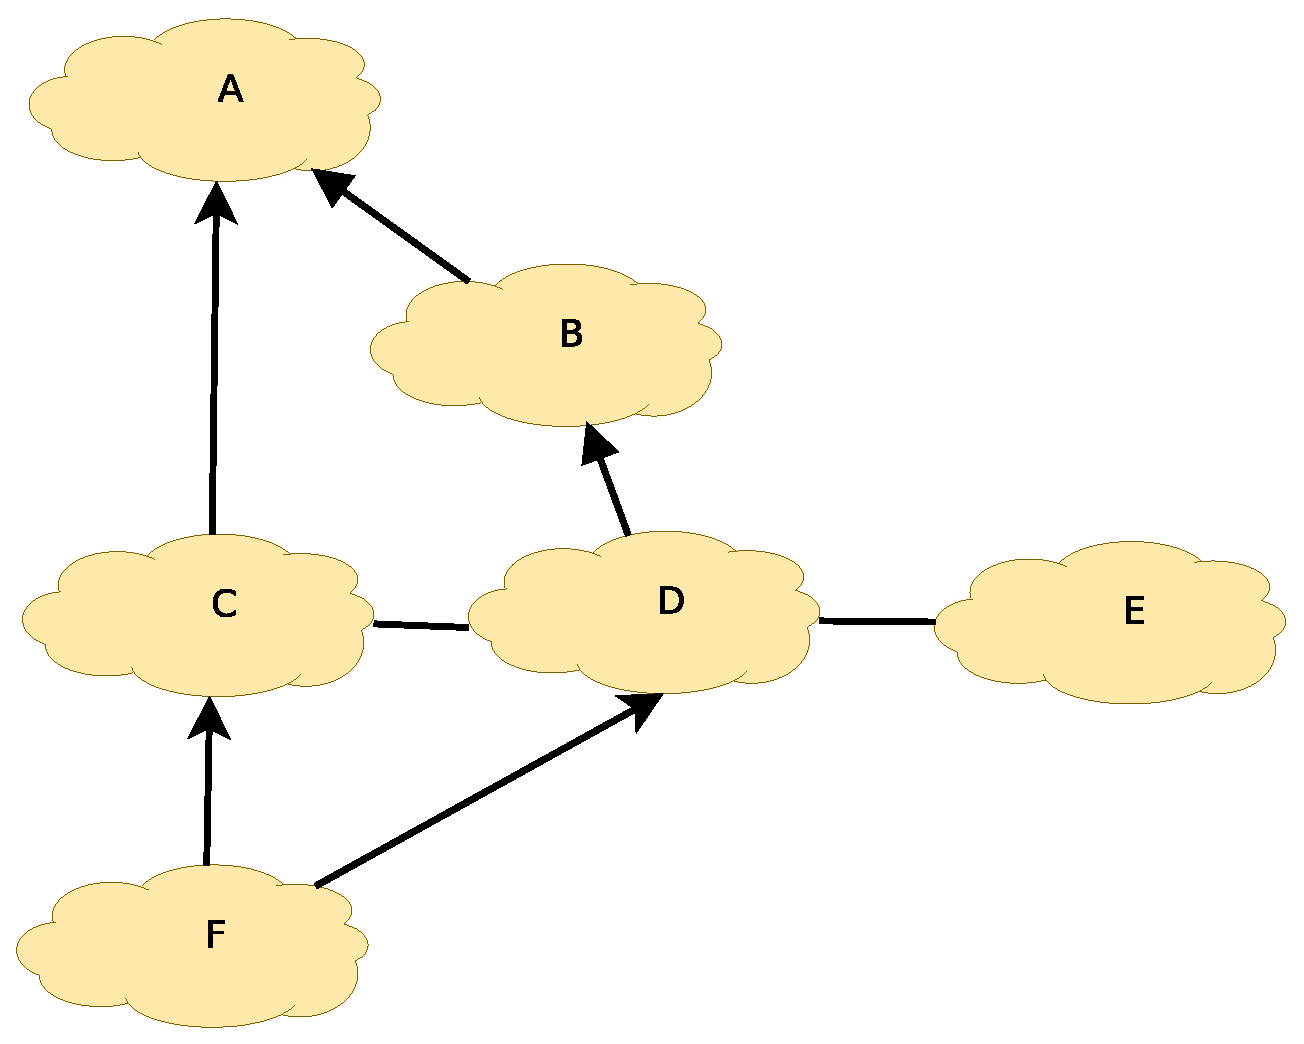
\includegraphics{bgp-as}}
\end{center}
\setcounter{partctr}{0}
\begin{list}{\bf\Alph{partctr}.}{\usecounter{partctr}}
\item Would the stub AS $F$ readvertise
  routes it learned from provider $C$ to its other provider, $D$?  Why
  or why not?
\item Would $E$ ever learn a route to a destination advertised by $F$?
  If so, what would be the AS path of the route it learned?  If not, why
  would it not learn a route?
\item If $A$ does not set any local preference values on routes that are
  advertised by $F$, and all ASes advertise routes according to common
  route export rules, then what is the AS path of the route that $A$
  will prefer to a destination that is advertised by $F$?
\item Suppose that AS $F$ wants AS $A$ to use the route $A B D F$ to
  reach an IP prefix that $F$ advertises.  Describe one way that AS $F$
  can try to cause AS $A$ to send traffic for the prefix along that
  path.  Will the approach guarantee that AS $A$ always chooses that
  path?  Why or why not?
\end{list}
~\ansbelow 
\vspace{2in}
\eprob

\sols{
\vspace{-1in}
\begin{answer}
\end{answer}
}

\newpage
\prob{8} Consider the router backplane below, with packets arriving as
shown.  The number on each packet designates its intended output port.
Suppose that each input and output port have a rate of 1 Gigabit per
second. 
\begin{center}
\resizebox{0.5\textwidth}{!}{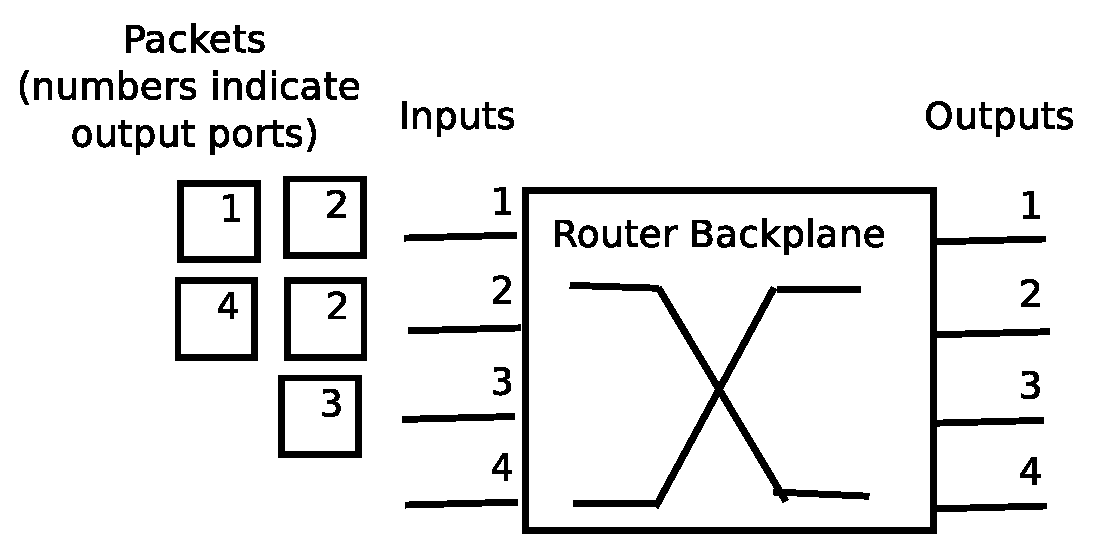
\includegraphics{backplane}}
\end{center}
\setcounter{partctr}{0}
\begin{list}{\bf\Alph{partctr}.}{\usecounter{partctr}}
\item Suppose the router has a {\bf {\em bus backplane}} with throughput of 5
  Gigabits per second.  What is the total maximum throughput that the
  router can achieve?  Why?
\item The example shows an example of {\em head-of-line blocking}.  Explain
  why, and explain how virtual output queueing can fix the problem.
\item Now suppose the router has a {\em crossbar switch backplane} with
  a throughput of 10 Gigabits per second (a ``speedup'' of 2) and virtual
  output queueing.  Given the packet arrival pattern shown in the
  figure, give a sequence of matchings of input ports to output ports
  that results in 100\% utilization (to save time, simple notation like
  ``Round 1: $1\rightarrow 2$'' is sufficient to indicate that you match
  input one to output two in round one).  Your solution should have two rounds.
\end{list}
~\ansbelow
\eprob

\newpage
\prob{5} Consider a link that has a capacity of 20 Mbps and receives
five traffic flows with respective demands: \{ 2 Mbps, 4 Mbps, 6 Mbps,
10 Mbps, 15 Mbps \}.  Suppose that the router wishes to allocate rates
to each of these flows in a {\em max-min} fair manner.  

Give the resulting max-min fair allocation of flows, in the form \{
$x_1$ Mbps, $x_2$ Mbps, ...\}, where $x_i$ are the resulting flow rates
in a max-min fair allocation.
~\ansbelow 
\vspace{2in}
\eprob

\sols{
\vspace{-1in}
\begin{answer}
\end{answer}
}

\prob{5} Consider the following longest prefix match forwarding table
for 4-bit addresses:
\begin{center}
\begin{tabular}{ll}
Prefix & Port \\ \hline
{\tt 0*} & A \\
{\tt 01*} & B \\
{\tt 0101} & C \\
{\tt 1*} & D \\
{\tt 111*} & E \\ \hline
\end{tabular}
\end{center}
\begin{enumerate}
\item Assuming longest prefix match, what port would be used for
  destination address {\tt 0111}?
\item Draw a simple {\em one-bit trie} representing the table.
\item Draw a simple {\em two-bit trie} representing the table.
\end{enumerate}

~\ansbelow 
\vspace{2in}
\eprob

\sols{
\vspace{-1in}
\begin{answer}
\end{answer}
}



\newpage
\prob{12} Consider the bridge topology shown the figure below. Assuming that
all of the forwarding tables are initially empty, write out the
forwarding tables at each of the four bridges $B_1$ through $B_4$ at the
conclusion of the following transmissions: 
\begin{center}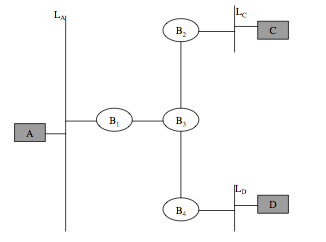
\includegraphics[width=0.5\linewidth]{lan-topo}\end{center}
\begin{itemize}
\item[1.] A sends to D 
\item[2.] D sends to A 
\item[3.] C sends to A
\end{itemize}
In the forwarding table at each node, identify the port by the unique
LAN segment ($L_A$, $L_C$, or $L_D$) reachable using that port, unless there
isn't one, in which case use the identifier of the neighboring bridge to
identify the port. 

{\bf After A sends to D:}

\begin{tabular}{|l|l||l|l||l|l||l|l|}
\multicolumn{2}{c}{\bf $B_1$} &
\multicolumn{2}{c}{\bf $B_2$} &
\multicolumn{2}{c}{\bf $B_3$} &
\multicolumn{2}{c}{\bf $B_4$} \\ \hline
Destination & Port & Destination & Port & Destination & Port &
Destination & Port \\ \hline
A & & A & & A & & A & \\
C & & C & & C & & C & \\
D & & D & & D & & D & \\
\hline
\end{tabular}


{\bf After D sends to A:}

\begin{tabular}{|l|l||l|l||l|l||l|l|}
\multicolumn{2}{c}{\bf $B_1$} &
\multicolumn{2}{c}{\bf $B_2$} &
\multicolumn{2}{c}{\bf $B_3$} &
\multicolumn{2}{c}{\bf $B_4$} \\ \hline
Destination & Port & Destination & Port & Destination & Port &
Destination & Port \\ \hline
A & & A & & A & & A & \\
C & & C & & C & & C & \\
D & & D & & D & & D & \\
\hline
\end{tabular}


{\bf After C sends to A:}

\begin{tabular}{|l|l||l|l||l|l||l|l|}
\multicolumn{2}{c}{\bf $B_1$} &
\multicolumn{2}{c}{\bf $B_2$} &
\multicolumn{2}{c}{\bf $B_3$} &
\multicolumn{2}{c}{\bf $B_4$} \\ \hline
Destination & Port & Destination & Port & Destination & Port &
Destination & Port \\ \hline
A & & A & & A & & A & \\
C & & C & & C & & C & \\
D & & D & & D & & D & \\
\hline
\end{tabular}


\eprob

\sols{
\vspace{-1in}
\begin{answer}
\end{answer}
}




\newpage
\section{Network Neutrality}

\prob{4} Define {\em network neutrality}.  Suppose that network
neutrality is {\em not} enforced.  Describe one benefit to users, one
benefit to ISPs, and one benefit to content providers.
~\ansbelow
\eprob
\vspace*{2in}

\prob{4} Explain why the lack of network neutrality might give an unfair
advantage to an ISP like Comcast, who also owns NBC, a major provider of
content such as television shows.
~\ansbelow 
\eprob



\newpage
\prob{8} A recent court ruling against the FCC suggested that although
ISPs did not need to remain neutral, they needed to be {\em
  transparent}, meaning that they would have to be clear about their
traffic prioritization and differential pricing policies.  

\begin{enumerate}
\item George Burdell wants to design a system to enforce transparency
  for ISPs in Atlanta.  He starts off by using a tool like {\tt iperf}
  (which you used in the assignments) to measure TCP throughput from his
  laptop at home to a server running in San Francisco.  He notices that
  the output of {\tt iperf} does not match the downstream throughput
  rate that his ISP advertises.  Ben Bitdiddle suggests that he should
  instead try using {\tt iperf} to a server that is located in Atlanta
  and he might see {\tt iperf} achieve a higher rate.  Is Ben right?
  Why or why not?
\item {\em Open-ended.} George begins sending traffic to the server in Atlanta and notices
  that {\tt iperf} {\em still} doesn't yield a throughput that is close
  to what his ISP advertises.  Ben suggests that other factors, such as
  George's laptop wireless card, the amount of load on his machine,
  ``cross traffic'' from other devices in his home, etc. may be
  interfering with George's measurement.  Help George make changes to
  his method that would better help isolate these effects.  {\em Hint:} You can
  consider collecting additional data, changing the vantage points that
  George is measuring to or from, and so forth.
\end{enumerate}
~\ansbelow \eprob


\newpage
\section{Bonus: Anonymous Course Feedback}

{\bf This page is anonymous.}  Rip this off from your exam, and turn it
in separately if you like.  You'll get five points for simply ripping
off the last page of the exam, but I'd prefer if you fill it out and
hand it in in a separate stack.  {\bf You can turn this page in at the next
class, or electronically (anonymously) on Piazza.}
\vspace{.5in}

What are the things you like most about the course so far?  Anything is
fair game here (topics, course structure, board technique, etc.).
\vspace{1.5in}


What are the things you like least about the course so far?  Again,
anything is fair game.
\vspace{1in}


What topics would you like to see covered?
\vspace{1in}




\label{lastpage}
\end{document}
